% Template adapted from https://github.com/jgm/pandoc-templates/blob/master/default.latex
% To be used with XeLaTex in memoiR
%%%%%%%%%%%%%%%%%%%%%%%%%%%%%%%%%%%%%%%%%%%%%%%%%%%%%%%%%%%%%%%%%%%%%%%%%%%%%%%%%%%%%%%%%

% Options for packages loaded elsewhere
\PassOptionsToPackage{unicode=true}{hyperref}
\PassOptionsToPackage{hyphens}{url}
\PassOptionsToPackage{dvipsnames,svgnames*,x11names*}{xcolor}
% Right to left support


\documentclass[
  10pt,
  italian,
  a4paper,
  extrafontsizes,onecolumn,openright
  ]{memoir}

% Double (or whatever) spacing

% Math
\usepackage{amssymb, amsmath}
% mathspec: arbitrary math fonts
\usepackage{unicode-math}
\defaultfontfeatures{Scale=MatchLowercase}
\defaultfontfeatures[\rmfamily]{Ligatures=TeX,Scale=1}

% Fonts
% \usepackage{lmodern}
\usepackage{fontspec}

% Main font
% Specific sanserif font
% Specific monotype font
\setmonofont[Scale=0.75]{Operator Mono SSm Book}
% Specific math font
% Chinese, Japanese, Corean fonts

% Use upquote for straight quotes in verbatim environments
\usepackage{upquote}
% Use microtype
\usepackage[]{microtype}
\UseMicrotypeSet[protrusion]{basicmath} % disable protrusion for tt fonts

% Verbatim in note

% Color links
\usepackage{xcolor}

% Strikeout

% Necessary for code chunks

% Listings package

% Tables
\usepackage{longtable,booktabs,tabu}
% Fix footnotes in tables (requires footnote package)
\IfFileExists{footnote.sty}{\usepackage{footnote}\makesavenoteenv{longtable}}{}

% Graphics
\usepackage{graphicx,grffile}
\graphicspath{{images/}}
\makeatletter
\def\maxwidth{\ifdim\Gin@nat@width>\linewidth\linewidth\else\Gin@nat@width\fi}
\def\maxheight{\ifdim\Gin@nat@height>\textheight\textheight\else\Gin@nat@height\fi}
\makeatother
% Scale images if necessary, so that they will not overflow the page
% margins by default, and it is still possible to overwrite the defaults
% using explicit options in \includegraphics[width, height, ...]{}
\setkeys{Gin}{width=\maxwidth,height=\maxheight,keepaspectratio}

% Prevent overfull lines
\setlength{\emergencystretch}{3em}  
\providecommand{\tightlist}{%
  \setlength{\itemsep}{0pt}\setlength{\parskip}{0pt}}

% Number sections for memoir (secnumdepth counter is ignored)
\setsecnumdepth{section}

% Set default figure placement to htbp
\makeatletter
\def\fps@figure{htbp}
\makeatother

% Spacing in lists
\usepackage{enumitem}

% Polyglossia
\usepackage{polyglossia}
\setmainlanguage{it}
\setotherlanguage{en-US}

% BibLaTeX
\usepackage[backend=biber,style=authoryear-ibid,isbn=false,backref=true,giveninits=true,uniquename=init,maxcitenames=2,maxbibnames=150,sorting=nyt,sortcites=false,style=apa]{biblatex}
\addbibresource{refs.bib}
\addbibresource{packages.bib}

% cslreferences environment required by pandoc > 2.7



%%%%%%%%%%%%%%%%%%%%%%%%%%%%%%%%%%%%%%%%%%%%%%%%%%%%%%%%%%
% memoiR format

% Chapter Summary environment 
\usepackage[tikz]{bclogo}
\newenvironment{Summary}
  {\begin{bclogo}[logo=\bctrombone, noborder=true, couleur=lightgray!50]{In breve}\parindent0pt}
  {\end{bclogo}}
% Syntax:
%
%```{block, type='Summary'}
% Deliver message here.
% ```

% scriptsize code 
\let\oldverbatim\verbatim
\def\verbatim{\oldverbatim\scriptsize}
% Applies to code blocks and R code results
% code chunk options size='scriptsize' applies only to R code and results
% if the code chunk sets a different size, \def\verbatim{...} is prioritary for code results 


% Layout
%%%%%%%%%%%%%%%%%%%%%%%%%%%%%%%%%%%%%%%%%%%%%%%%%%%%%%%%%%

% Based on memoir, style companion
\newcommand{\MemoirChapStyle}{daleif1}
\newcommand{\MemoirPageStyle}{Ruled}

% Space between paragraphs
\usepackage{parskip}
  \abnormalparskip{3pt}

% Adjust margin paragraphs vertical position
\usepackage{marginfix}


% Margins
%%%%%%%%%%%%%%%%%%%%%%%%%%%%%%%%%%%%%%%

% allow use of '-',+','/' ans '*' to make simple length computation
\usepackage{calc}

% Full-width figures utilities
\newlength\widthw % full width
\newlength{\rf}
\newcommand*{\definesHSpace}{
  \strictpagecheck % slower but efficient detection of odd/even pages
  \checkoddpage
  \ifoddpage
  \setlength{\rf}{0mm}
  \else
  \setlength{\rf}{\marginparsep+\marginparwidth}
  \fi
}

\makeatletter
% 1" margins for the front matter.
\newcommand*{\SmallMargins}{
  \setlrmarginsandblock{1.5in}{1.5in}{*}
  \setmarginnotes{0.1in}{0.1in}{0.1in}
 \setulmarginsandblock{1.5in}{1in}{*}
  \checkandfixthelayout
  \ch@ngetext
  \clearpage
  \setlength{\widthw}{\textwidth+\marginparsep+\marginparwidth}
  \footnotesatfoot
  \chapterstyle{\MemoirChapStyle}  % Chapter and page styles must be recalled
  \pagestyle{\MemoirPageStyle}
}

% 3" outer margin for the main matter
\newcommand{\LargeMargins}{\SmallMargins}
\makeatother

% Figure captions and footnotes in outer margins


% Main title page with filigrane
%%%%%%%%%%%%%%%%%%%%%%%%%%%%%%%%%%%%%%%%%%%%%%%%%%%%%%%%%%

% Text blocks
\usepackage[absolute,overlay]{textpos}
  \setlength{\TPHorizModule}{1mm}
  \setlength{\TPVertModule}{1mm}

\newcommand{\MainTitlePage}[2]{
  \SmallMargins % Margins
  \pagestyle{empty} % No header/footer
  \textblockorigin{\stockwidth-\paperwidth-\trimedge}{\trimtop} % recto
  \begin{textblock*}{2mm}(\spinemargin/2,\uppermargin/2)
    \rule{1pt}{\paperheight-\uppermargin}
  \end{textblock*}
  \begin{textblock*}{\paperwidth*2/3}(\paperwidth/5, \paperheight/5)
    \flushright
    \begin{Spacing}{3}
      {\fontfamily{qtm}\selectfont\fontsize{45}{45}\selectfont\textsc{\thetitle}}
    \end{Spacing}
  \end{textblock*}
    \begin{textblock*}{\paperwidth*2/3}(\paperwidth/5, \paperheight/2)
    \flushright
    {\fontfamily{qtm}\huge\theauthor}
  \end{textblock*}
    \begin{textblock*}{\paperwidth*2/3}[0, 1](\spinemargin, \uppermargin+\textheight)
    \normalfont\thedate
  \end{textblock*}
  ~\\ % Print a character or the page will not exist
  \newpage
  \textblockorigin{\trimedge}{\trimtop} % verso
  \begin{textblock*}{\textwidth}(\paperwidth-\spinemargin-\textwidth, \uppermargin)
    #1
  \end{textblock*}
  \begin{textblock*}{\textwidth}[0,1](\paperwidth-\spinemargin-\textwidth, \uppermargin+\textheight+\footskip)
    \centering
    
\includegraphics[width=\paperwidth/4]{logo}\\ \bigskip
    #2
  \end{textblock*}
  ~\\ % Print a character or the page will not exist
  \newpage
}

% Clear page and open an even one (\clearpage opens an odd one)
\newcommand{\evenpage}{
  \clearpage
  \strictpagecheck % slower but efficient detection of odd/even pages
  \checkoddpage
  \ifoddpage
    \thispagestyle{empty}
    ~\\ % Print a character or the page will not exist
    \newpage
  \else
    % do nothing
  \fi
}


%% PDF title page to insert
%%%%%%%%%%%%%%%%%%%%%%%%%%%%%%%%%%%%%%%%%%%%%%%%%%%%%%%%%%



%% Bibliography
%%%%%%%%%%%%%%%%%%%%%%%%%%%%%%%%%%%%%%%%%%%%%%%%%%%%%%%%%%

\usepackage[strict,autostyle]{csquotes}
% Repeated citation as author-year-title instead of author-title (modification of footcite:note in verbose-inote.cbx)

%% Table of Contents
%%%%%%%%%%%%%%%%%%%%%%%%%%%%%%%%%%%%%%%%%%%%%%%%%%%%%%%%%%

% fix the typesetting of the part number
\renewcommand\partnumberlinebox[2]{#2\ ---\ }


% Fonts
%%%%%%%%%%%%%%%%%%%%%%%%%%%%%%%%%%%%%%%%%%%%%%%%%%%%%%%%%%


% Hyperref comes last
%%%%%%%%%%%%%%%%%%%%%%%%%%%%%%%%%%%%%%%%%%%%%%%%%%%%%%%%%%

\usepackage{hyperref}
\hypersetup{
  pdftitle={Psicometria},
  pdfauthor={Corrado Caudek},
  colorlinks=true,
  linkcolor=Maroon,
  citecolor=Blue,
  urlcolor=Blue,
  breaklinks=true}

% Don't use monospace font for urls
\urlstyle{same}


% Title, author, date from YAML to LaTeX
%%%%%%%%%%%%%%%%%%%%%%%%%%%%%%%%%%%%%%%%%%%%%%%%%%%%%%%%%%

\title{Psicometria}

\author{Corrado Caudek}

\date{2022-01-12}


% Include headers (preamble.tex) here
%%%%%%%%%%%%%%%%%%%%%%%%%%%%%%%%%%%%%%%%%%%%%%%%%%%%%%%%%%
% Add LaTeX code into the preamble of the document here
\hyphenation{bio-di-ver-si-ty sap-lings}


%%%%%%%%%%%%%%%%%%%%%%%%%%%%%%%%%%%%%%%%%%%%%%%%%%%%%%%%%%%%%%%%%%%%%%%%%
% memoiR dalef3 chapter style 
% https://ctan.crest.fr/tex-archive/info/latex-samples/MemoirChapStyles/MemoirChapStyles.pdf
\usepackage{amsmath}

\usepackage{soul}
\definecolor{nicered}{rgb}{.647,.129,.149}

\makeatletter
\makechapterstyle{pedersen}
\makeatother

\DeclareMathOperator{\Var}{Var} % Define variance operator
\DeclareMathOperator{\SD}{SD} % Define sd operator
\DeclareMathOperator{\Cov}{Cov} % Define covariance operator
\DeclareMathOperator{\Corr}{Corr} % Define correlation operator
\DeclareMathOperator{\Me}{Me} % Define mediane operator
\DeclareMathOperator{\Mo}{Mo} % Define mode operator
\DeclareMathOperator{\Bin}{Bin} % Define binomial operator
\DeclareMathOperator{\Bernoulli}{Bernoulli} % Define Bernoulli operator
\DeclareMathOperator{\Poi}{Poi} % Define Poisson operator
\DeclareMathOperator{\Uniform}{Uniform} % Define Uniform operator
\DeclareMathOperator{\Cauchy}{Cauchy} % Define Cauchy operator
\DeclareMathOperator{\elpd}{elpd} % Define elpd operator
\DeclareMathOperator{\lppd}{lppd} % Define lppd operator
\DeclareMathOperator{\LOO}{LOO} % Define LOO operator
\DeclareMathOperator{\Ber}{\mathscr{B}} % Define Bernoulli operator
\DeclareMathOperator{\B}{B} % beta function
% \mbox{B}(a, b) % beta function
% \mbox{Beta}(a, b) % beta distribution
\newcommand{\R}{\textsf{R}} % Define R programming language symbol
\newcommand{\E}{\mathbb{E}} % Define expected value operator
\newcommand{\Real}{\mathbb{R}} % Define real number operator
\newcommand{\Prob}{\mathscr{P}}
\DeclareMathOperator{\argmin}{arg\,min} % thin space, limits on side in displays
\DeclareMathOperator{\argmax}{arg\,max} % no space, limits on side in displays

\raggedbottom % allow variable (ragged) site heights
\frenchspacing

\usepackage[
  labelfont=bf, 
  font={small, it} 
]{caption} 
\usepackage{upquote} % print correct quotes in verbatim-environments
\usepackage{empheq} 
\usepackage{xfrac}
%\usepackage{lstbayes}
%\usepackage{awesomebox}



\usepackage{booktabs}
\usepackage{longtable}
\usepackage{array}
\usepackage{multirow}
\usepackage{wrapfig}
\usepackage{float}
\usepackage{colortbl}
\usepackage{pdflscape}
\usepackage{tabu}
\usepackage{threeparttable}
\usepackage{threeparttablex}
\usepackage[normalem]{ulem}
\usepackage{makecell}
\usepackage{xcolor}


% End of preamble
%%%%%%%%%%%%%%%%%%%%%%%%%%%%%%%%%%%%%%%%%%%%%%%%%%%%%%%%%%


\begin{document}
\frontmatter

% Title page
%%%%%%%%%%%%%%%%%%%%%%%%%%%%%%%%%%%%%%%%%%%%%%%%%%%%%%%%%%


\MainTitlePage{Questo documento è stato realizzato con:

\begin{itemize}
  \item \LaTeX\; e la classe memoir (\url{http://www.ctan.org/pkg/memoir});
  \item $\R$ (\url{http://www.r-project.org/}) e RStudio (\url{http://www.rstudio.com/});
  \item bookdown (\url{http://bookdown.org/}) e memoiR (\url{https://ericmarcon.github.io/memoiR/}).
  \end{itemize}}{Nel blog della mia pagina personale sono forniti alcuni approfondimenti degli argomenti qui trattati.
\url{https://ccaudek.github.io/caudeklab/}}


% Before Body
%%%%%%%%%%%%%%%%%%%%%%%%%%%%%%%%%%%%%%%%%%%%%%%%%%%%%%%%%%





% Contents
%%%%%%%%%%%%%%%%%%%%%%%%%%%%%%%%%%%%%%%%%%%%%%%%%%%%%%%%%%

\LargeMargins
{
\hypersetup{linkcolor=}
\setcounter{tocdepth}{3}
\tableofcontents
}


% Body
%%%%%%%%%%%%%%%%%%%%%%%%%%%%%%%%%%%%%%%%%%%%%%%%%%%%%%%%%%

\LargeMargins
\scriptsize

\normalsize

\chapter*{}

\vfill

\scriptsize

\normalsize

Data della versione presente: Gennaio 12, 2022.

\hypertarget{prefazione}{%
\chapter{Prefazione}\label{prefazione}}

\emph{Data Science per psicologi} contiene il materiale delle lezioni dell'insegnamento di \emph{Psicometria B000286} (A.A. 2021/2022) rivolto agli studenti del primo anno del Corso di Laurea in Scienze e Tecniche Psicologiche dell'Università degli Studi di Firenze. \emph{Psicometria} si propone di fornire agli studenti un'introduzione all'analisi dei dati in psicologia. Le conoscenze/competenze che verranno sviluppate in questo insegnamento sono quelle della Data science, ovvero un insieme di conoscenze/competenze che si pongono all'intersezione tra statistica (ovvero, richiedono la capacità di comprendere teoremi statistici) e informatica (ovvero, richiedono la capacità di sapere utilizzare un software).

\hypertarget{la-psicologia-e-la-data-science}{%
\section{La psicologia e la Data science}\label{la-psicologia-e-la-data-science}}

\begin{quote}
\emph{It's worth noting, before getting started, that this material is hard. If you find yourself confused at any point, you are normal. Any sense of confusion you feel is just your brain correctly calibrating to the subject matter. Over time, confusion is replaced by comprehension {[}\ldots{]}}

\hfill --- Richard McElreath
\end{quote}

Sembra sensato spendere due parole su un tema che è importante per gli studenti: quello indicato dal titolo di questo Capitolo. È ovvio che agli studenti di psicologia la statistica non piace. Se piacesse, forse studierebbero Data science e non psicologia; ma non lo fanno. Di conseguenza, gli studenti di psicologia si chiedono: ``perché dobbiamo perdere tanto tempo a studiare queste cose quando in realtà quello che ci interessa è tutt'altro?'' Questa è una bella domanda.

C'è una ragione molto semplice che dovrebbe farci capire perché la Data science è così importante per la psicologia. Infatti, a ben pensarci, la psicologia è una disciplina intrinsecamente statistica, se per statistica intendiamo quella disciplina che studia la variazione delle caratteristiche degli individui nella popolazione. La psicologia studia \emph{gli individui} ed è proprio la variabilità inter- e intra-individuale ciò che vogliamo descrivere e, in certi casi, predire. In questo senso, la psicologia è molto diversa dall'ingegneria, per esempio. Le proprietà di un determinato ponte sotto certe condizioni, ad esempio, sono molto simili a quelle di un altro ponte, sotto le medesime condizioni. Quindi, per un ingegnere la statistica è poco importante: le proprietà dei materiali sono unicamente dipendenti dalla loro composizione e restano costanti. Ma lo stesso non può dirsi degli individui: ogni individuo è unico e cambia nel tempo. E le variazioni tra gli individui, e di un individuo nel tempo, sono l'oggetto di studio proprio della psicologia: è dunque chiaro che i problemi che la psicologia si pone sono molto diversi da quelli affrontati, per esempio, dagli ingegneri. Questa è la ragione per cui abbiamo tanto bisogno della Data science in psicologia: perché la Data science ci consente di descrivere la variazione e il cambiamento. E queste sono appunto le caratteristiche di base dei fenomeni psicologici.

Sono sicuro che, leggendo queste righe, a molti studenti sarà venuta in mente la seguente domanda: perché non chiediamo a qualche esperto di fare il ``lavoro sporco'' (ovvero le analisi statistiche) per noi, mentre noi (gli psicologi) ci occupiamo solo di ciò che ci interessa, ovvero dei problemi psicologici slegati dai dettagli ``tecnici'' della Data science? La risposta a questa domanda è che non è possibile progettare uno studio psicologico sensato senza avere almeno una comprensione rudimentale della Data science. Le tematiche della Data science non possono essere ignorate né dai ricercatori in psicologia né da coloro che svolgono la professione di psicologo al di fuori dell'Università. Infatti, anche i professionisti al di fuori dall'università non possono fare a meno di leggere la letteratura psicologica più recente: il continuo aggiornamento delle conoscenze è infatti richiesto dalla deontologia della professione. Ma per potere fare questo è necessario conoscere un bel po' di Data science! Basta aprire a caso una rivista specialistica di psicologia per rendersi conto di quanto ciò sia vero: gli articoli che riportano i risultati delle ricerche psicologiche sono zeppi di analisi statistiche e di modelli formali. E la comprensione della letteratura psicologica rappresenta un requisito minimo nel bagaglio professionale dello psicologo.

Le considerazioni precedenti cercano di chiarire il seguente punto: la Data science non è qualcosa da studiare a malincuore, in un singolo insegnamento universitario, per poi poterla tranquillamente dimenticare. Nel bene e nel male, gli psicologi usano gli strumenti della Data science in tantissimi ambiti della loro attività professionale: in particolare quando costruiscono, somministrano e interpretano i test psicometrici. È dunque chiaro che possedere delle solide basi di Data science è un tassello imprescindibile del bagaglio professionale dello psicologo. In questo insegnamento verrano trattati i temi base della Data science e verrà adottato un punto di vista bayesiano, che corrisponde all'approccio più recente e sempre più diffuso in psicologia.

\hypertarget{come-studiare}{%
\section{Come studiare}\label{come-studiare}}

\begin{quote}
\emph{I know quite certainly that I myself have no special talent. Curiosity, obsession and dogged endurance, combined with self-criticism, have brought me to my ideas.}

\hfill --- Albert Einstein
\end{quote}

Il giusto metodo di studio per prepararsi all'esame di Psicometria è quello di seguire attivamente le lezioni, assimilare i concetti via via che essi vengono presentati e verificare in autonomia le procedure presentate a lezione. Incoraggio gli studenti a farmi domande per chiarire ciò che non è stato capito appieno. Incoraggio gli studenti a utilizzare i forum attivi su Moodle e, soprattutto, a svolgere gli esercizi proposti su Moodle. I problemi forniti su Moodle rappresentano il livello di difficoltà richiesto per superare l'esame e consentono allo studente di comprendere se le competenze sviluppate fino a quel punto sono sufficienti rispetto alle richieste dell'esame.

La prima fase dello studio, che è sicuramente individuale, è quella in cui è necessario acquisire le conoscenze teoriche relative ai problemi che saranno presentati all'esame. La seconda fase di studio, che può essere facilitata da scambi con altri e da incontri di gruppo, porta ad acquisire la capacità di applicare le conoscenze: è necessario capire come usare un software (\(\textsf{R}\)) per applicare i concetti statistici alla specifica situazione del problema che si vuole risolvere. Le due fasi non sono però separate: il saper fare molto spesso ci aiuta a capire meglio.

\hypertarget{sviluppare-un-metodo-di-studio-efficace}{%
\section*{Sviluppare un metodo di studio efficace}\label{sviluppare-un-metodo-di-studio-efficace}}
\addcontentsline{toc}{section}{Sviluppare un metodo di studio efficace}

\begin{quote}
\emph{Memorization is not learning.}

\hfill --- Richard Phillips Feynman
\end{quote}

Avendo insegnato molte volte in passato un corso introduttivo di analisi dei dati ho notato nel corso degli anni che gli studenti con l'atteggiamento mentale che descriverò qui sotto generalmente ottengono ottimi risultati. Alcuni studenti sviluppano naturalmente questo approccio allo studio, ma altri hanno bisogno di fare uno sforzo per maturarlo. Fornisco qui sotto una breve descrizione del ``metodo di studio'' che, nella mia esperienza, è il più efficace per affrontare le richieste di questo insegnamento \autocite{burger20125}.

\begin{itemize}
\tightlist
\item
  Dedicate un tempo sufficiente al materiale di base, apparentemente facile; assicuratevi di averlo capito bene. Cercate le lacune nella vostra comprensione. Leggere presentazioni diverse dello stesso materiale (in libri o articoli diversi) può fornire nuove intuizioni.
\item
  Gli errori che facciamo sono i nostri migliori maestri. Istintivamente cerchiamo di dimenticare subito i nostri errori. Ma il miglior modo di imparare è apprendere dagli errori che commettiamo. In questo senso, una soluzione corretta è meno utile di una soluzione sbagliata. Quando commettiamo un errore questo ci fornisce un'informazione importante: ci fa capire qual è il materiale di studio sul quale dobbiamo ritornare e che dobbiamo capire meglio.
\item
  C'è ovviamente un aspetto ``psicologico'' nello studio. Quando un esercizio o problema ci sembra incomprensibile, la cosa migliore da fare è dire: ``mi arrendo'', ``non ho idea di cosa fare!''. Questo ci rilassa: ci siamo già arresi, quindi non abbiamo niente da perdere, non dobbiamo più preoccuparci. Ma non dobbiamo fermarci qui. Le cose ``migliori'' che faccio (se ci sono) le faccio quando non ho voglia di lavorare. Alle volte, quando c'è qualcosa che non so fare e non ho idea di come affontare, mi dico: ``oggi non ho proprio voglia di fare fatica'', non ho voglia di mettermi nello stato mentale per cui ``in 10 minuti devo risolvere il problema perché dopo devo fare altre cose''. Però ho voglia di \emph{divertirmi} con quel problema e allora mi dedico a qualche aspetto ``marginale'' del problema, che so come affrontare, oppure considero l'aspetto più difficile del problema, quello che non so come risolvere, ma invece di cercare di risolverlo, guardo come altre persone hanno affrontato problemi simili, opppure lo stesso problema in un altro contesto. Non mi pongo l'obiettivo ``risolvi il problema in 10 minuti'', ma invece quello di farmi un'idea ``generale'' del problema, o quello di capire un caso più specifico e più semplice del problema. Senza nessuna pressione. Infatti, in quel momento ho deciso di non lavorare (ovvero, di non fare fatica). Va benissimo se ``parto per la tangente'', ovvero se mi metto a leggere del materiale che sembra avere poco a che fare con il problema centrale (le nostre intuizioni e la nostra curiosità solitamente ci indirizzano sulla strada giusta). Quando faccio così, molto spesso trovo la soluzione del problema che mi ero posto e, paradossalmente, la trovo in un tempo minore di quello che, in precedenza, avevo dedicato a ``lavorare'' al problema. Allora perché non faccio sempre così? C'è ovviamente l'aspetto dei ``10 minuti'' che non è sempre facile da dimenticare. Sotto pressione, possiamo solo agire in maniera automatica, ovvero possiamo solo applicare qualcosa che già sappiamo fare. Ma se dobbiamo imparare qualcosa di nuovo, la pressione è un impedimento.
\item
  È utile farsi da soli delle domande sugli argomenti trattati, senza limitarsi a cercare di risolvere gli esercizi che vengono assegnati. Quando studio qualcosa mi viene in mente: ``se questo è vero, allora deve succedere quest'altra cosa''. Allora verifico se questo è vero, di solito con una simulazione. Se i risultati della simulazione sono quelli che mi aspetto, allora vuol dire che ho capito. Se i risultati sono diversi da quelli che mi aspettavo, allora mi rendo conto di non avere capito e ritorno indietro a studiare con più attenzione la teoria che pensavo di avere capito -- e ovviamente mi rendo conto che c'era un aspetto che avevo frainteso. Questo tipo di verifica è qualcosa che dobbiamo fare da soli, in prima persona: nessun altro può fare questo al posto nostro.
\item
  Non aspettatevi di capire tutto la prima volta che incontrate un argomento nuovo.\footnote{Ricordatevi inoltre che gli individui tendono a sottostimare la propria capacità di apprendere \autocite{horn2021underestimating}.} È utile farsi una nota mentalmente delle lacune nella vostra comprensione e tornare su di esse in seguito per carcare di colmarle. L'atteggiamento naturale, quando non capiamo i dettagli di qualcosa, è quello di pensare: ``non importa, ho capito in maniera approssimativa questo punto, non devo preoccuparmi del resto''. Ma in realtà non è vero: se la nostra comprensione è superficiale, quando il problema verrà presentato in una nuova forma, non riusciremo a risolverlo. Per cui i dubbi che ci vengono quando studiamo qualcosa sono il nostro alleato più prezioso: ci dicono esattamente quali sono gli aspetti che dobbiamo approfondire per potere migliorare la nostra preparazione.
\item
  È utile sviluppare una visione d'insieme degli argomenti trattati, capire l'obiettivo generale che si vuole raggiungere e avere chiaro il contributo che i vari pezzi di informazione forniscono al raggiungimento di tale obiettivo. Questa organizzazione mentale del materiale di studio facilita la comprensione. È estremamente utile creare degli schemi di ciò che si sta studiando. Non aspettate che sia io a fornirvi un riepilogo di ciò che dovete imparare: sviluppate da soli tali schemi e tali riassunti.
\item
  Tutti noi dobbiamo imparare l'arte di trovare le informazioni, non solo nel caso di questo insegnamento. Quando vi trovate di fronte a qualcosa che non capite, o ottenete un oscuro messaggio di errore da un software, ricordatevi: ``Google is your friend''.
\end{itemize}

\bigskip

Corrado Caudek

\mainmatter

\hypertarget{appendix-appendix}{%
\appendix}


\hypertarget{simbologia-di-base}{%
\chapter{Simbologia di base}\label{simbologia-di-base}}

Per una scrittura più sintetica possono essere utilizzati alcuni simboli
matematici.

\begin{itemize}
\tightlist
\item
  \(\log(x)\): il logaritmo naturale di \(x\).
\item
  L'operatore logico booleano \(\land\) significa ``e'' (congiunzione
  forte) mentre il connettivo di disgiunzione \(\lor\) significa ``o''
  (oppure) (congiunzione debole).
\item
  Il quantificatore esistenziale \(\exists\) vuol dire ``esiste almeno
  un'' e indica l'esistenza di almeno una istanza del concetto/oggetto
  indicato. Il quantificatore esistenziale di unicità \(\exists!\)
  (``esiste soltanto un'') indica l'esistenza di esattamente una istanza
  del concetto/oggetto indicato. Il quantificatore esistenziale
  \(\nexists\) nega l'esistenza del concetto/oggetto indicato.
\item
  Il quantificatore universale \(\forall\) vuol dire ``per ogni.''
\item
  \(\mathcal{A, S}\): insiemi.
\item
  \(x \in A\): \(x\) è un elemento dell'insieme \(A\).
\item
  L'implicazione logica ``\(\Rightarrow\)'' significa ``implica'' (se
  \ldots allora). \(P \Rightarrow Q\) vuol dire che \(P\) è condizione
  sufficiente per la verità di \(Q\) e che \(Q\) è condizione necessaria
  per la verità di \(P\).
\item
  L'equivalenza matematica ``\(\iff\)'' significa ``se e solo se'' e indica
  una condizione necessaria e sufficiente, o corrispondenza biunivoca.
\item
  Il simbolo \(\vert\) si legge ``tale che.''
\item
  Il simbolo \(\triangleq\) (o \(:=\)) si legge ``uguale per definizione.''
\item
  Il simbolo \(\Delta\) indica la differenza fra due valori della
  variabile scritta a destra del simbolo.
\item
  Il simbolo \(\propto\) si legge ``proporzionale a.''
\item
  Il simbolo \(\approx\) si legge ``circa.''
\item
  Il simbolo \(\in\) della teoria degli insiemi vuol dire ``appartiene'' e
  indica l'appartenenza di un elemento ad un insieme. Il simbolo
  \(\notin\) vuol dire ``non appartiene.''
\item
  Il simbolo \(\subseteq\) si legge ``è un sottoinsieme di'' (può
  coincidere con l'insieme stesso). Il simbolo \(\subset\) si legge ``è
  un sottoinsieme proprio di.''
\item
  Il simbolo \(\#\) indica la cardinalità di un insieme.
\item
  Il simbolo \(\cap\) indica l'intersezione di due insiemi. Il simbolo
  \(\cup\) indica l'unione di due insiemi.
\item
  Il simbolo \(\emptyset\) indica l'insieme vuoto o evento impossibile.
\item
  In matematica, \(\mbox{argmax}\) identifica l'insieme dei punti per i quali una data funzione raggiunge il suo massimo. In altre parole, \(\mbox{argmax}_x f(x)\) è l'insieme dei valori di \(x\) per i quali \(f(x)\) raggiunge il valore più alto.
\item
  \(a, c, \alpha, \gamma\): scalari.
\item
  \(\boldsymbol{x}, \boldsymbol{y}\): vettori.
\item
  \(\boldsymbol{X}, \boldsymbol{Y}\): matrici.
\item
  \(X \sim p\): la variabile casuale \(X\) si distribuisce come \(p\).
\item
  \(p(\cdot)\): distribuzione di massa o di densità di probabilità.
\item
  \(p(y \mid \boldsymbol{x})\): la probabilità o densità di \(y\) dato \(\boldsymbol{x}\), ovvero \(p(y = \boldsymbol{Y} \mid x = \boldsymbol{X})\).
\item
  \(f(x)\): una funzione arbitraria di \(x\).
\item
  \(f(\boldsymbol{X}; \theta, \gamma)\): \(f\) è una funzione di \(\boldsymbol{X}\) con parametri \(\theta, \gamma\). Questa notazione indica che \(\boldsymbol{X}\) sono i dati che vengono passati ad un modello di parametri \(\theta, \gamma\).
\item
  \(\mathcal{N}(\mu, \sigma^2)\): distribuzione gaussiana di media \(\mu\) e varianza \(sigma^2\).
\item
  \(\mbox{Beta}(\alpha, \beta)\): distribuzione Beta di parametri \(\alpha\) e \(\beta\).
\item
  \(\mathcal{U}(a, b)\): distribuzione uniforme con limite inferiore \(a\) e limite superiore \(b\).
\item
  \(\mbox{Cauchy}(\alpha, \beta)\): distribuzione di Cauchy di parametri \(\alpha\) (posizione: media) e \(\beta\) (scala: radice quadrata della varianza).
\item
  \(\mathcal{B}(p)\): distribuzione di Bernoulli di parametro \(p\) (probabilità di successo).
\item
  \(\mbox{Bin}(n, p)\): distribuzione binomiale di parametri \(n\) (numero di prove) e \(p\) (probabilità di successo).
\item
  \(\mathbb{KL} (p \mid\mid q)\): la divergenza di Kullback-Leibler da \(p\) a \(q\).
\end{itemize}

\hypertarget{introduzione-al-linguaggio-r}{%
\chapter{Introduzione al linguaggio R}\label{introduzione-al-linguaggio-r}}

In questa sezione della dispensa saranno presentate le caratteristiche di base e la filosofia dell'ambiente \texttt{R}, passando poi a illustrare le strutture dati e le principali strutture di controllo. Verranno introdotte alcune funzioni utili per la gestione dei dati e verranno forniti i rudimenti per realizzare semplici funzioni. Verranno introdotti i tipi di file editabili in RStudio (script, markdown, \ldots). Nello specifico, dopo aver accennato alcune caratteristiche del sistema \texttt{tidyverse}, verranno illustrate le principali funzionalità dell'IDE RStudio e dei pacchetti \texttt{dplyr} e \texttt{ggplot2}. Sul web sono disponibili tantissime introduzioni all'uso di \texttt{R} come, ad esempio, \href{https://rstudio-education.github.io/hopr/}{Hands-On Programming with R}, \href{https://r4ds.had.co.nz}{R for Data Science}, \href{https://bookdown.org/hneth/ds4psy/}{Data Science for Psychologists}, e \href{https://bookdown.org/hneth/i2ds/}{Introduction to Data Science}.

\hypertarget{prerequisiti}{%
\section{Prerequisiti}\label{prerequisiti}}

Al fine di utilizzare \texttt{R} è necessario eseguire le seguenti tre operazioni
nell'ordine dato:

\begin{enumerate}
\def\labelenumi{\arabic{enumi}.}
\tightlist
\item
  Installare \texttt{R};
\item
  Installare RStudio;
\item
  Installare R-Packages (se necessario).
\end{enumerate}

Di seguito viene descritto come installare \texttt{R} e RStudio.

\hypertarget{installare-r-e-rstudio}{%
\subsection{Installare R e RStudio}\label{installare-r-e-rstudio}}

\(\R\) è disponibile gratuitamente ed è scaricabile dal sito
\url{http://www.rproject.org/}. Dalla pagina principale del sito
\texttt{r-project.org} andiamo sulla sezione \texttt{Download} e scegliamo un server a
piacimento per scaricare il software d'installazione. Una volta
scaricato l'installer, lo installiamo come un qualsiasi software,
cliccando due volte sul file d'istallazione. Esistono versioni di \(\R\) per
tutti i più diffusi sistemi operativi (Windows, Mac OS X e Linux).

Il R Core Development Team lavora continuamente per migliorare le
prestazioni di \(\R\), per correggere errori e per consentire l'uso di con
nuove tecnologie. Di conseguenza, periodicamente vengono rilasciate
nuove versioni di \(\R\). Informazioni a questo proposito sono fornite sulla
pagina web \url{https://www.r-project.org/}. Per installare una nuova
versione di \(\R\) si segue la stessa procedura che è stata seguita per la
prima installazione.

Insieme al software si possono scaricare dal sito principale sia manuali d'uso che numerose dispense per approfondire diversi aspetti di \(\R\). In particolare, nel sito \url{http://cran.r-project.org/other-docs.html} si possono trovare anche numerose dispense in italiano (sezione ``Other languages'').

Dopo avere installato \(\R\) è opportuno installare anche RStudio. RStudio si
può scaricare da \url{https://www.rstudio.com/}. Anche RStudio è disponibile
per tutti i più diffusi sistemi operativi.

\hypertarget{utilizzare-rstudio-per-semplificare-il-lavoro}{%
\subsection{Utilizzare RStudio per semplificare il lavoro}\label{utilizzare-rstudio-per-semplificare-il-lavoro}}

Possiamo pensare ad \(\R\) come al motore di un automobile e a RStudio come
al cruscotto di un automobile. Più precisamente, \(\R\) è un linguaggio di
programmazione che esegue calcoli mentre RStudio è un ambiente di
sviluppo integrato (IDE) che fornisce un'interfaccia grafica aggiungendo
una serie di strumenti che facilitano la fase di sviluppo e di
esecuzione del codice. Utilizzeremo dunque \(\R\) mediante RStudio. In altre
parole,

\textbf{non aprite}


\includegraphics[width=0.15\textwidth,height=\textheight]{images/Rlogo.png}

\textbf{aprite invece}


\includegraphics[width=0.3\textwidth,height=\textheight]{images/RStudio-Logo-Blue-Gradient.png}

L'ambiente di lavoro di RStudio è costituito da quattro finestre: la finestra del codice (scrivere-eseguire script), la finestra della console (riga di comando -
output), la finestra degli oggetti (elenco oggetti-cronologia dei
comandi) e la finestra dei pacchetti-dei grafici-dell'aiuto in linea.

\begin{figure}
\hypertarget{fig:rstudio_pics}{%
\centering
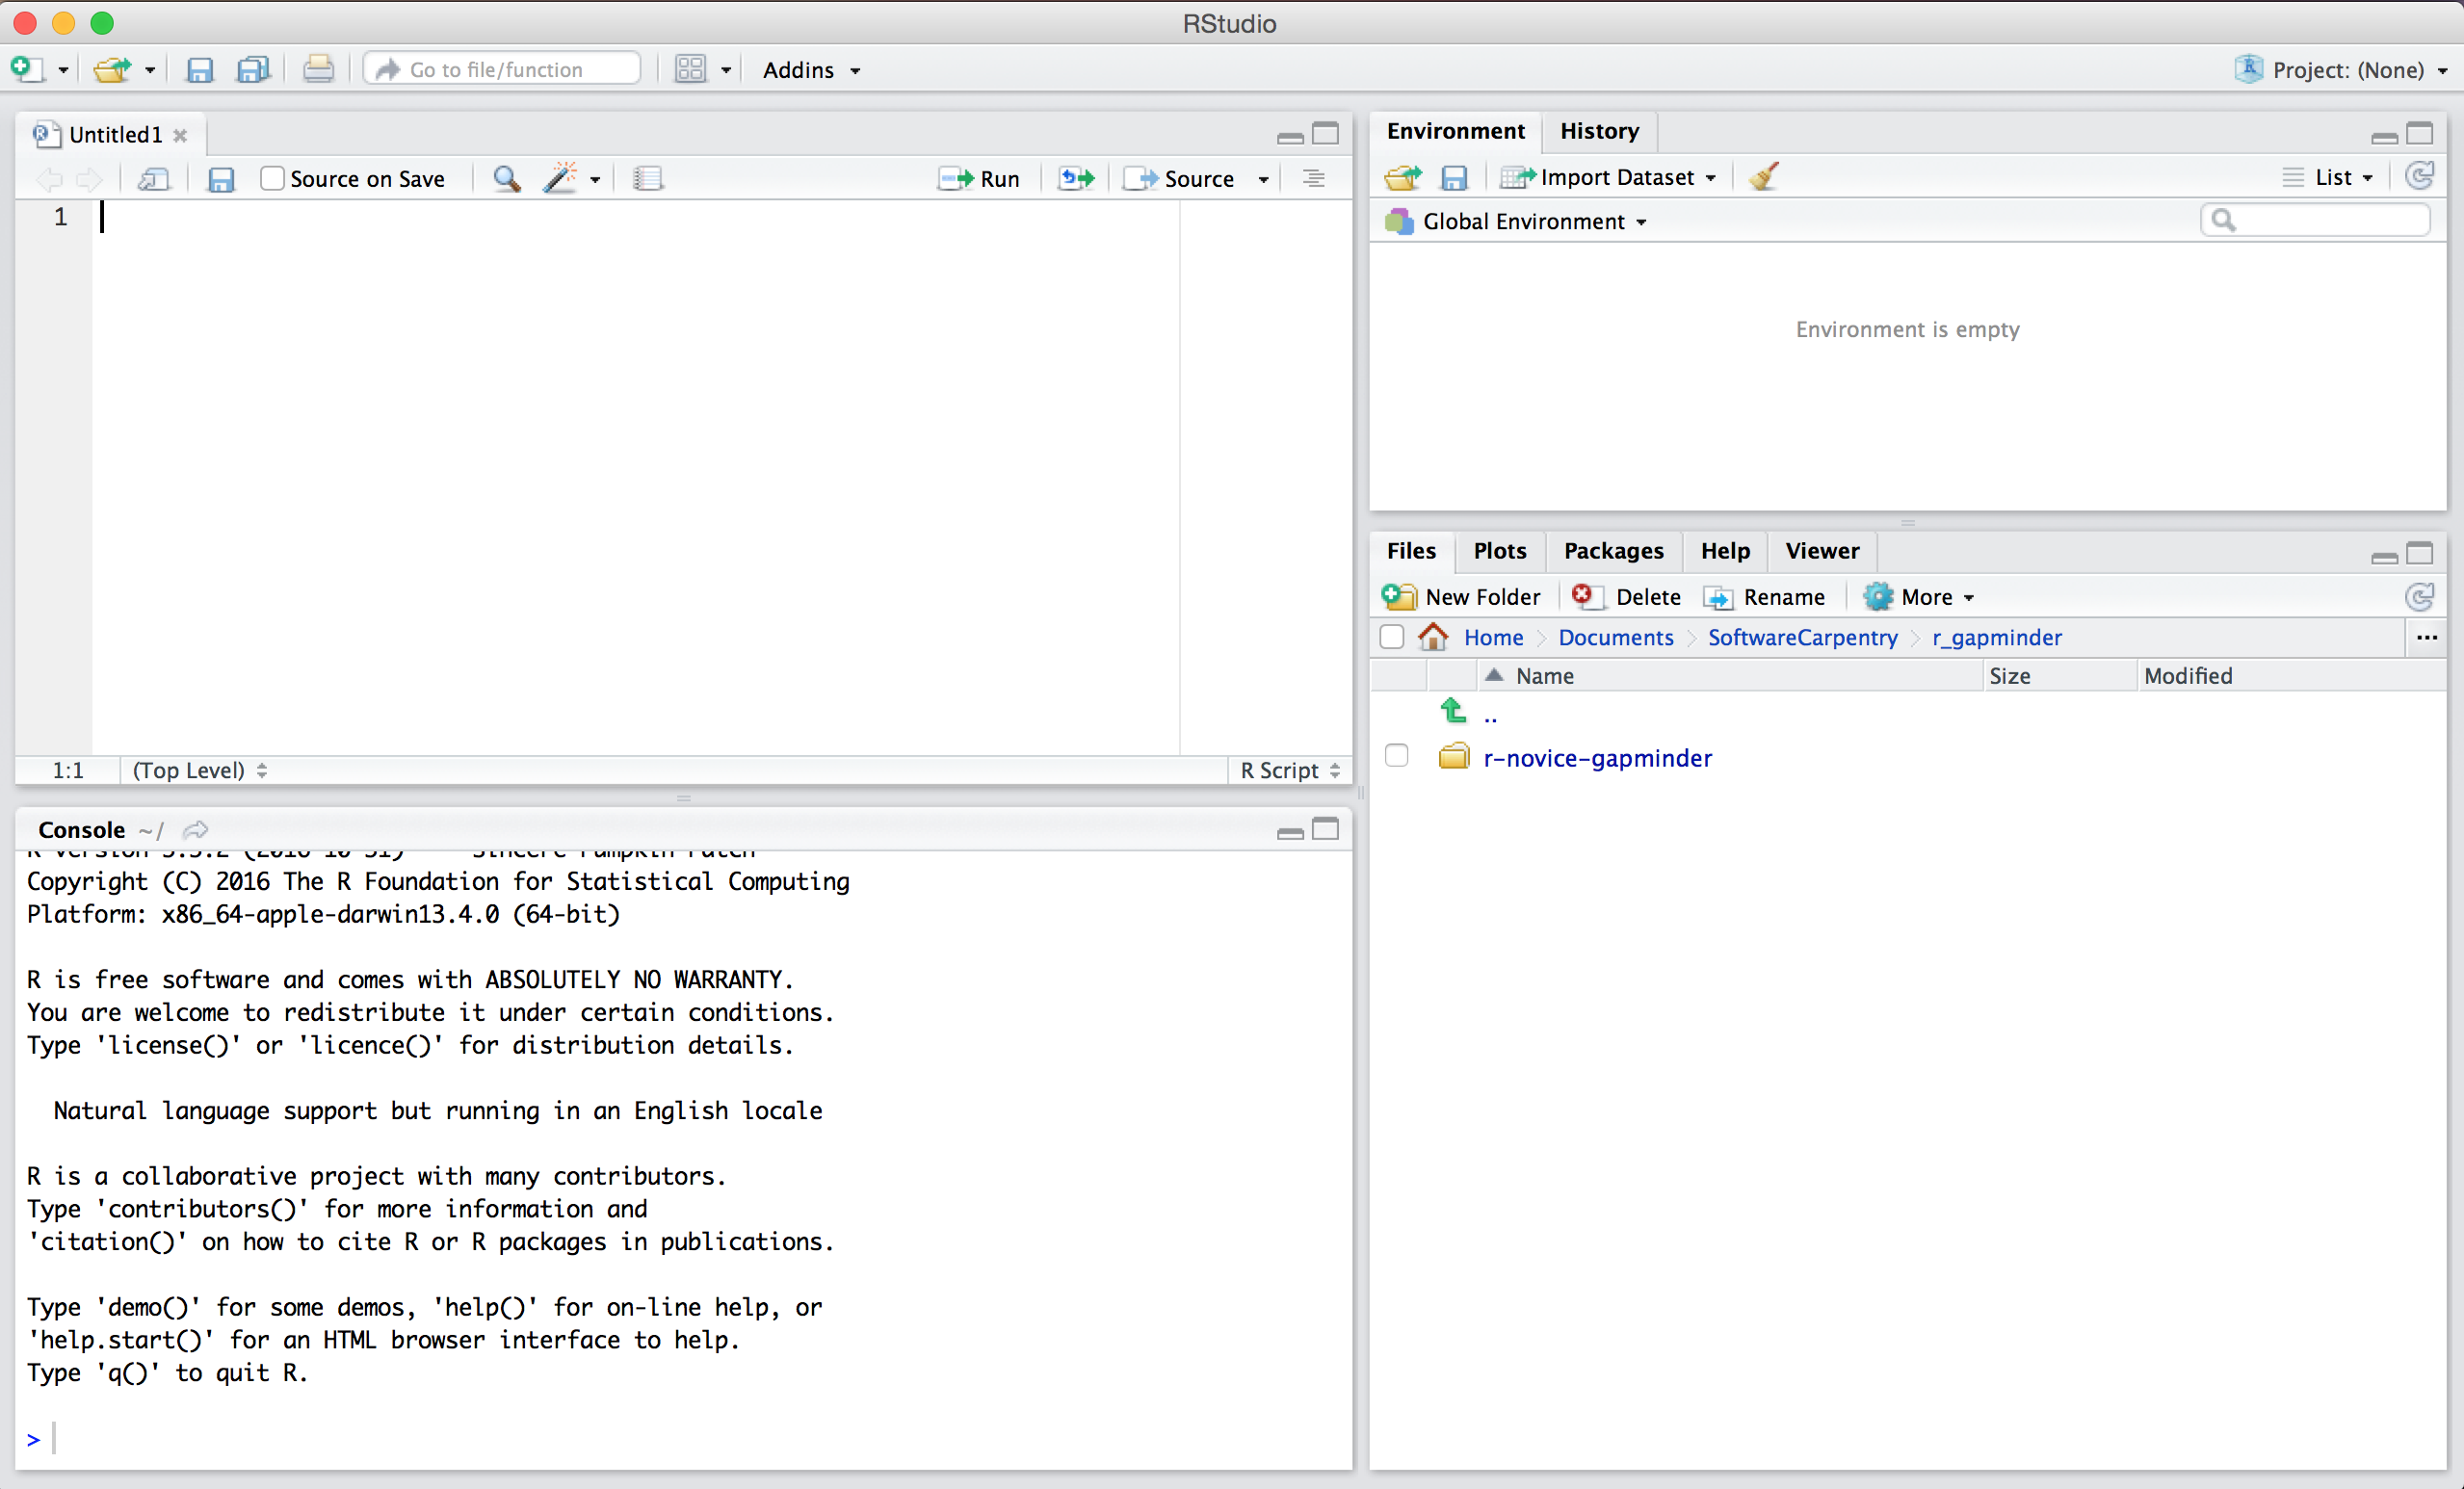
\includegraphics[width=1\textwidth,height=\textheight]{images/rstudio_pics.png}
\caption{La console di RStudio.}\label{fig:rstudio_pics}
}
\end{figure}

\hypertarget{eseguire-il-codice}{%
\subsection{Eseguire il codice}\label{eseguire-il-codice}}

Mediante il menu a tendina di RStudio, scegliendo il percorso

\begin{verbatim}
File > New File > R Notebook
\end{verbatim}

oppure

\begin{verbatim}
File > New File > R Script
\end{verbatim}

l'utente può aprire nella finestra del codice (in alto a destra) un \(\R\) Notebook o un \(\R\) script dove inserire le istruzioni da eseguire.

In un \(\R\) script, un blocco di codice viene eseguito selezionando un
insieme di righe di istruzioni e digitando la sequenza di tasti
\texttt{Command} + \texttt{Invio} sul Mac, oppure \texttt{Control} + \texttt{Invio} su Windows. In
un R Notebook, un blocco di codice viene eseguito schiacciando il
bottone con l'icona \(\color{red}\blacktriangleright\) (``Run current
chunk'') posizionata a destra rispetto al codice.

\hypertarget{installare-cmdstan}{%
\section{\texorpdfstring{Installare \texttt{cmdstan}}{Installare cmdstan}}\label{installare-cmdstan}}

È possibile installare \texttt{cmdstan} in almento tre modi. Per informazioni dettagliate, si vedano le istruzioni \href{https://mc-stan.org/docs/2_28/cmdstan-guide/cmdstan-installation.html}{CmdStan Installation}.

Prima di installare \texttt{cmdstan}, tre raccomandazioni generali:

\begin{itemize}
\tightlist
\item
  usare la versione più recente del sistema operativo;
\item
  usare la versione più recente di RStudio;
\item
  usare la versione più recente di \(\R\).
\end{itemize}

Se i tre vincoli precedenti sono soddisfatti, l'installazione di \texttt{cmdstan} dovrebbe procedere senza intoppi. Altrimenti si possono creare dei problemi di non facile soluzione.

Il modo più semplice per installare \texttt{cmdstan} è quello di installare prima \href{https://mc-stan.org/cmdstanr/}{cmdstanr} per poi utilizzare le funzionalità di quel pacchetto per l'installazione di \texttt{cmdstan}.

Un secondo metodo (che è quello che io uso normalmente) è quello di installare dal sorgente, seguendo le istruzioni riportante su \href{https://mc-stan.org/docs/2_28/cmdstan-guide/cmdstan-installation.html}{CmdStan Installation}.

Un terzo metodo (che richiede una minima comprensione delle funzionalità della shell e di Python) richiede, avendo prima installato \href{https://www.anaconda.com/products/individual}{Anaconda}, di digitare sulla console del proprio computer (la shell) le seguenti istruzioni:

\begin{verbatim}
conda create -n stan-env -c conda-forge cmdstan
conda activate stan-env
\end{verbatim}

Su \texttt{macos}, prima di installare \texttt{cmdstan}, è necessario installare la versione più recente di Xcode. Dopo avere installato Xcode, aprire la app. Verrà chiesto all'utente se si vogliono istallare delle componenti aggiuntive. Questo passaggio è cruciale, perché senza queste componenti aggiuntive \texttt{cmdstan} non funzionerà. Dopo avere installato le componenti aggiuntive, aprire Xcode e, in caso, accettare i termini della licenza. A quel punto si può chiudere Xcode. Ogni volta che Xcode viene aggiornato (deve sempre essere aggiornato quando un aggiornamento è disponibile), queste operazioni vanno ripetute.


% Bibliography
%%%%%%%%%%%%%%%%%%%%%%%%%%%%%%%%%%%%%%%%%%%%%%%%%%%%%%%%%%

\backmatter
\SmallMargins

\printbibliography
\onecolumn


% Tables (of tables, of figures)
%%%%%%%%%%%%%%%%%%%%%%%%%%%%%%%%%%%%%%%%%%%%%%%%%%%%%%%%%%


\cleardoublepage
\LargeMargins
\listoffigures


% After-body (LaTeX code inclusion)
%%%%%%%%%%%%%%%%%%%%%%%%%%%%%%%%%%%%%%%%%%%%%%%%%%%%%%%%%%




% Back cover
%%%%%%%%%%%%%%%%%%%%%%%%%%%%%%%%%%%%%%%%%%%%%%%%%%%%%%%%%%%

% Even page, small margins, no running head, no page number.
\evenpage
\SmallMargins
\thispagestyle{empty}

\begin{normalsize}

\begin{description}

\selectlanguage{italian}
\item[Abstract]
This document contains the material of the lessons of Psicometria B000286 (2021/2022) aimed at students of the first year of the Degree Course in Psychological Sciences and Techniques of the University of Florence, Italy.
\item[Keywords]
Data science, Bayesian statistics.
~\\

\end{description}

\end{normalsize}


\end{document}
